\documentclass[10pt,twocolumn]{IEEEtran}


% correct bad hyphenation here
\hyphenation{op-tical net-works semi-conduc-tor}

\usepackage{amsmath,graphicx,amsfonts,amssymb,amsthm,epsfig,mathrsfs,balance}
\usepackage{subcaption,tikz,color,multirow,algorithm,algpseudocode,algorithmicx}
\usepackage{cite,url,framed,bm,dsfont,lipsum}

\setlength{\tabcolsep}{1.1pt}

\newtheorem{assumption}{Assumption}
\newtheorem{theorem}{Theorem}
\newtheorem{corollary}[theorem]{Corollary}
\newtheorem{definition}{Definition}
\newtheorem{lemma}{Lemma}
\newtheorem{proposition}{Proposition}
\newtheorem{remark}{Remark}
\newtheorem{property}{Property}
\newtheorem{example}{Example}

\newcommand{\differential}{{\rm{d}}}

\renewcommand*{\thefootnote}{\fnsymbol{footnote}}
\newcommand{\red}{\color{red}}



\begin{document}

\title{\LARGE \bf Stochastic Uncertainty Propagation in Power System Dynamics using Meausre-valued Proximal Recursions}


\author{First~Author,~\IEEEmembership{Member,~IEEE,}
        Second~Author,~\IEEEmembership{Fellow,~OSA,}
        and~Third~Author,~\IEEEmembership{Life~Fellow,~IEEE}% <-this % stops a space
\thanks{M. Shell was with the Department
of Electrical and Computer Engineering, Georgia Institute of Technology, Atlanta,
GA, 30332 USA e-mail: (see http://www.michaelshell.org/contact.html).}% <-this % stops a space
\thanks{A. Halder is with the Department of Applied Mathematics, University of California, Santa Cruz, CA 95064, USA, {\texttt{\{ahalder\}@ucsc.edu}}. This research was partially supported by the NSF award 1923278.}}% <-this % stops a space
%\thanks{Manuscript received April 19, 2005; revised August 26, 2015.}}
% The paper headers
%\markboth{Journal of \LaTeX\ Class Files,~Vol.~14, No.~8, August~2015}%

\maketitle

\begin{abstract}
The abstract goes here.
\end{abstract}

\begin{IEEEkeywords}
Uncertainty propagation, power system dynamics, optimal transport, proximal operator.
\end{IEEEkeywords}



\section{Introduction}
\IEEEPARstart{T}{his} demo file is intended to serve as a ``starter file''
for IEEE journal papers \lipsum[3-5]







\section{Conclusion}
The conclusion goes here.


\appendices
\section{Proof of the First Zonklar Equation}
Appendix one text goes here.

% you can choose not to have a title for an appendix
% if you want by leaving the argument blank
\section{}
Appendix two text goes here.


% use section* for acknowledgment
\section*{Acknowledgment}


\begin{figure}
\centering
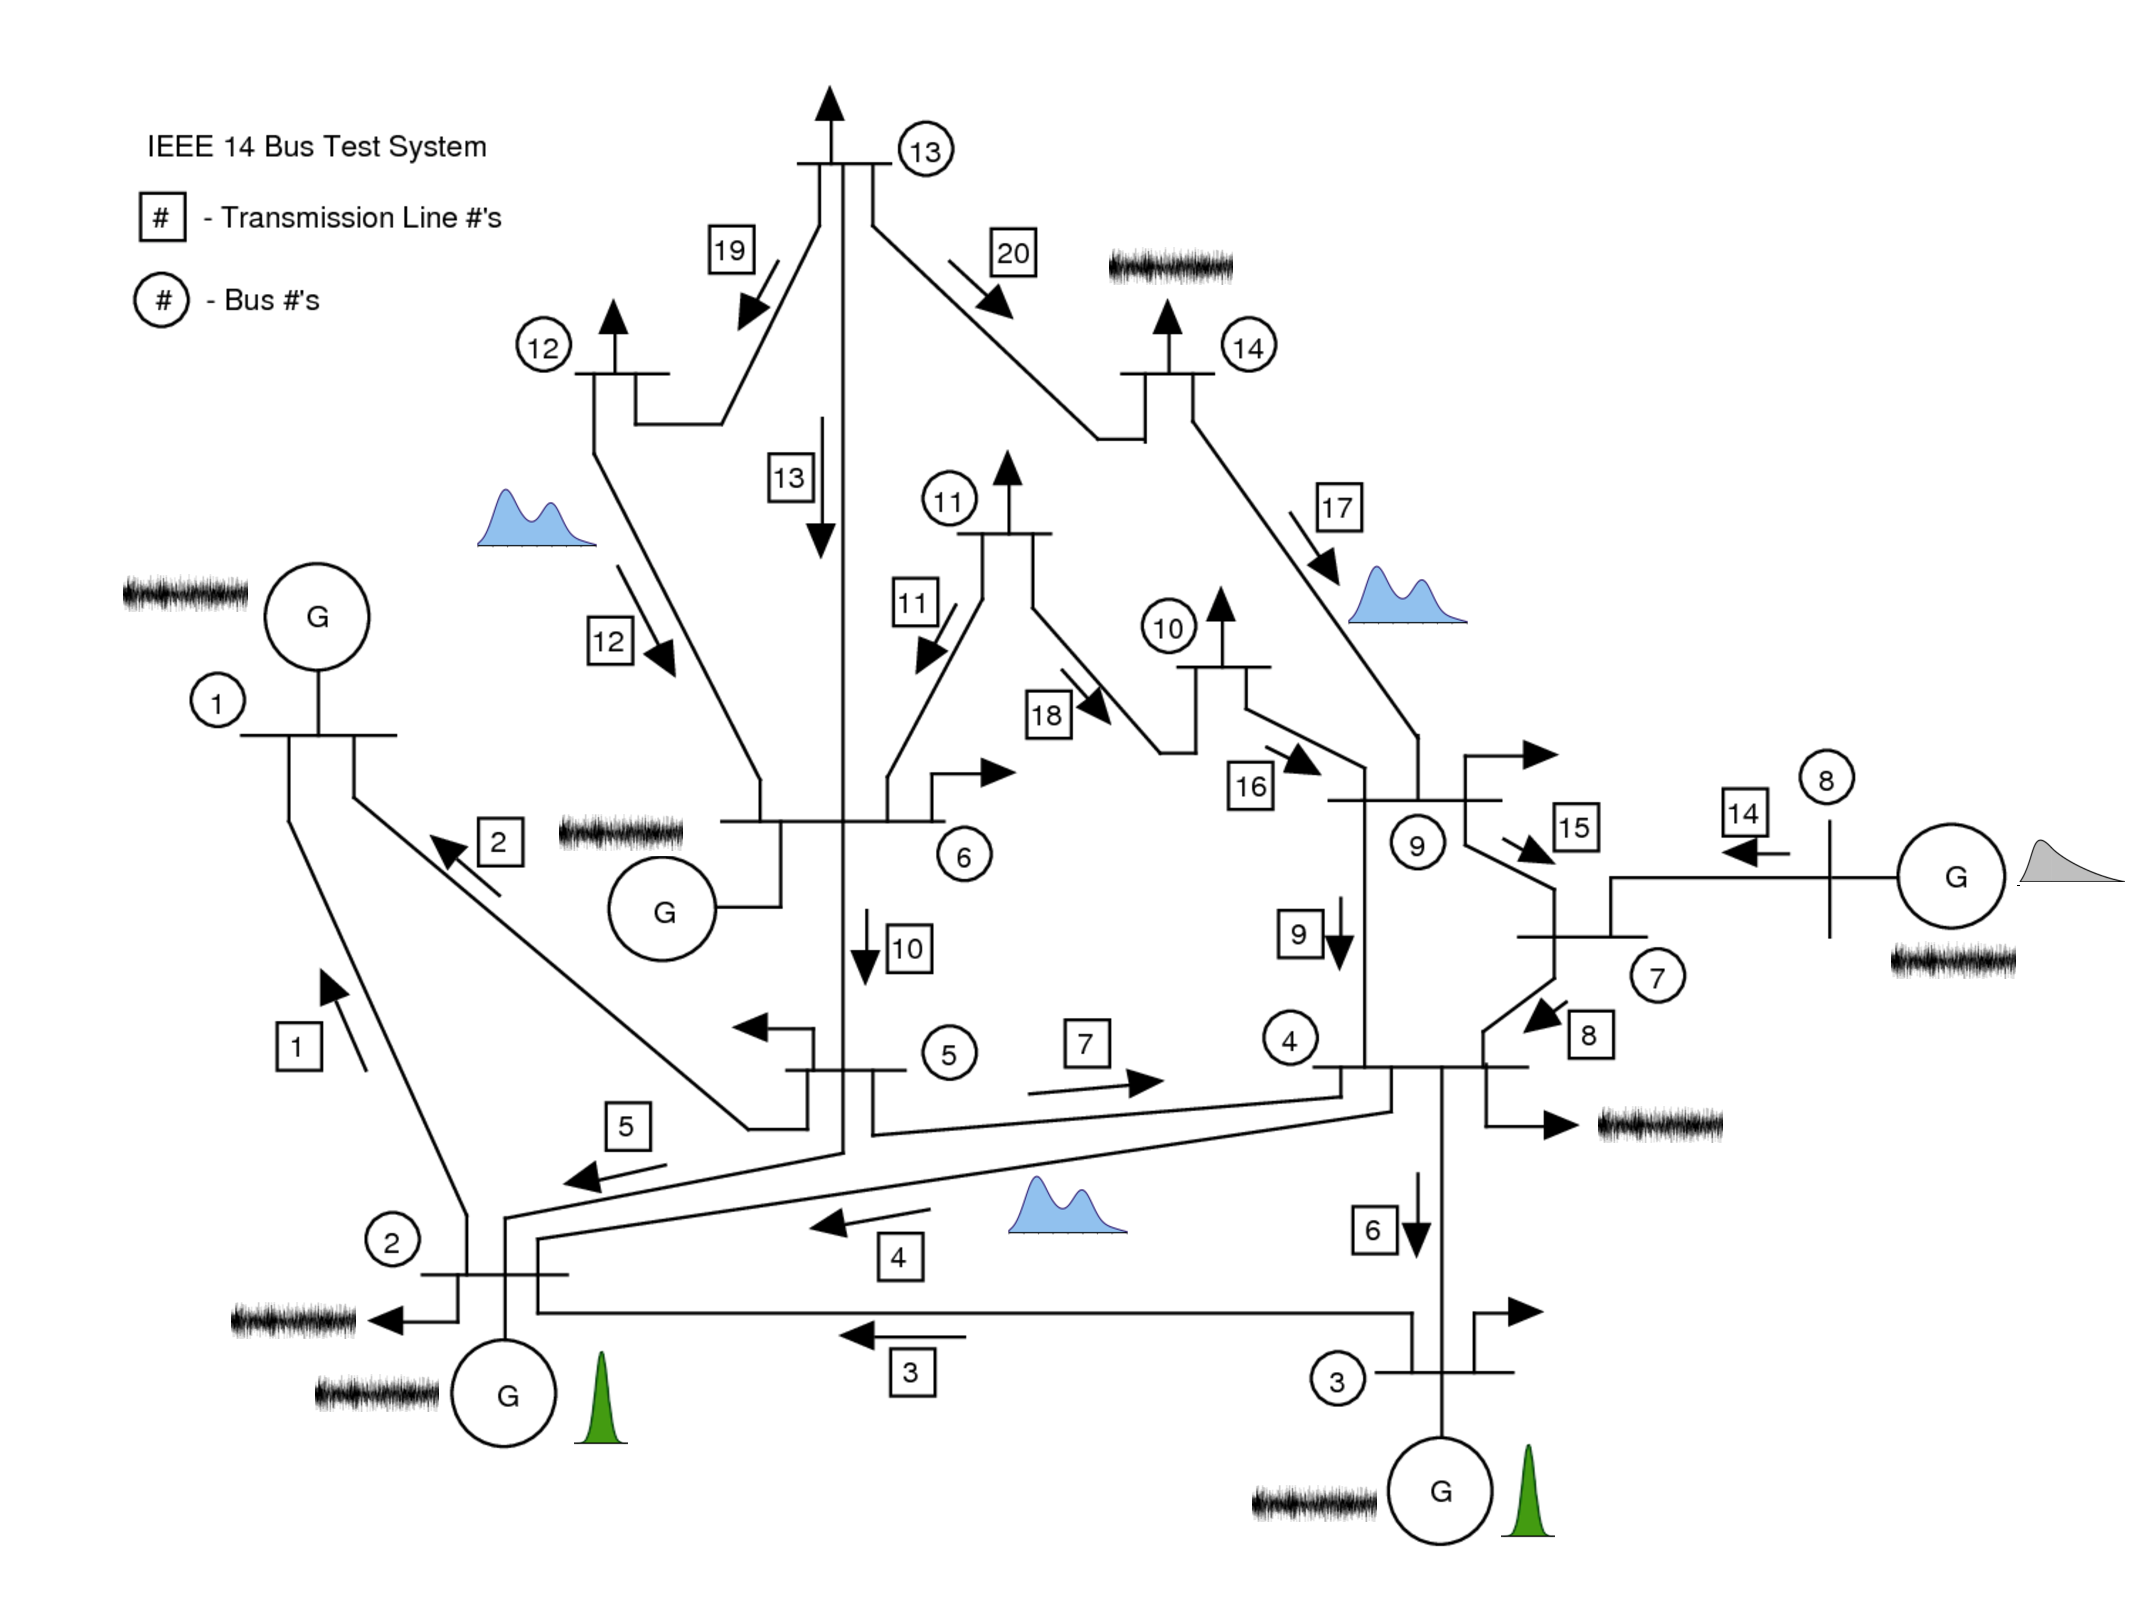
\includegraphics[width=\linewidth]{IEEE14BusWithUnc.pdf}
\caption{\small{A schematic of the IEEE 14 bus test system with stochastic uncertainties. The Uncertainty sources may include stochastic forcing and parametric uncertainties at some generators, random variabilities at some loads, and parametric uncertainties along some transmission lines. For depiction purposes, we indicated the parametric uncertainties as PDFs, and stochastic forcing as intermittent signals.}}
\label{fig:Motivating}
\end{figure}


\begin{figure}
\centering
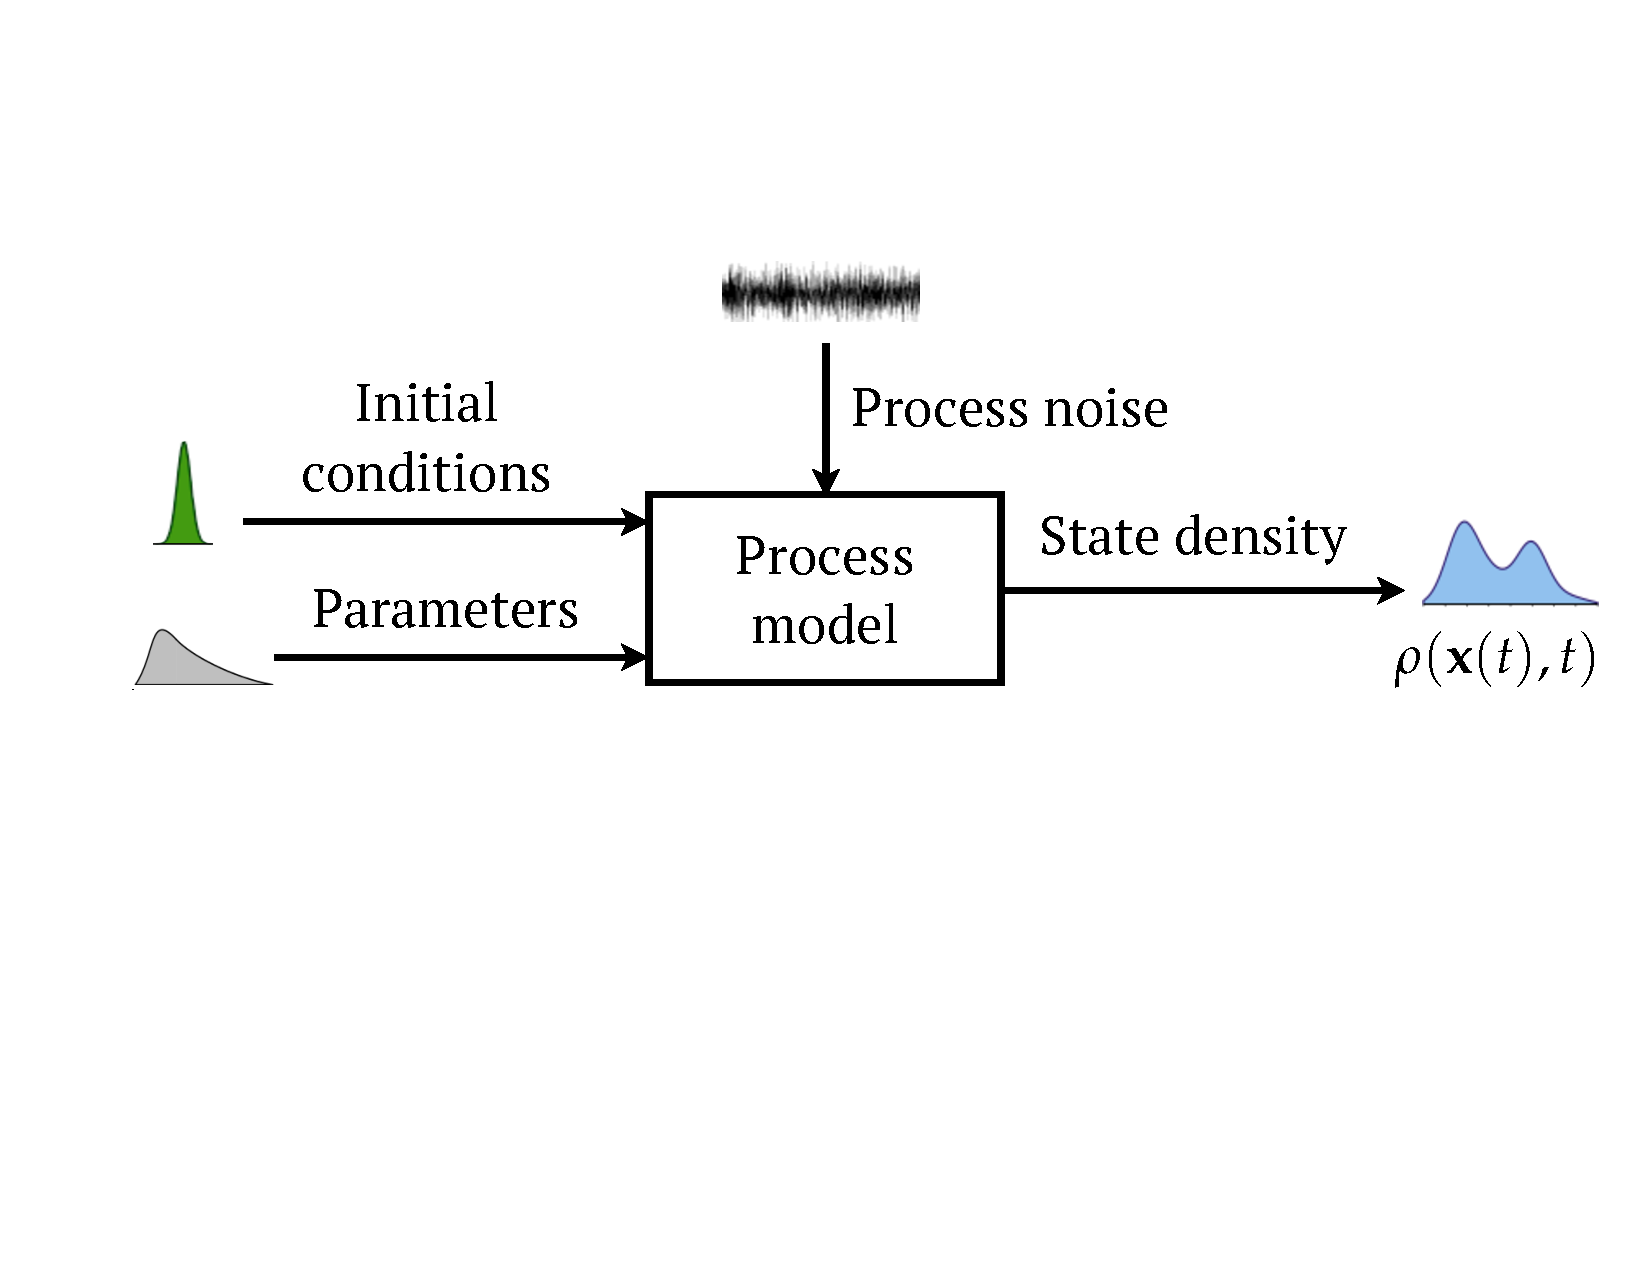
\includegraphics[width=0.9\linewidth]{UncPropBlockDiagm.pdf}
\caption{\small{Block diagram for joint state PDF propagation.}}
\label{fig:UncertaintyPropagation}
\end{figure}

\begin{figure}
\centering
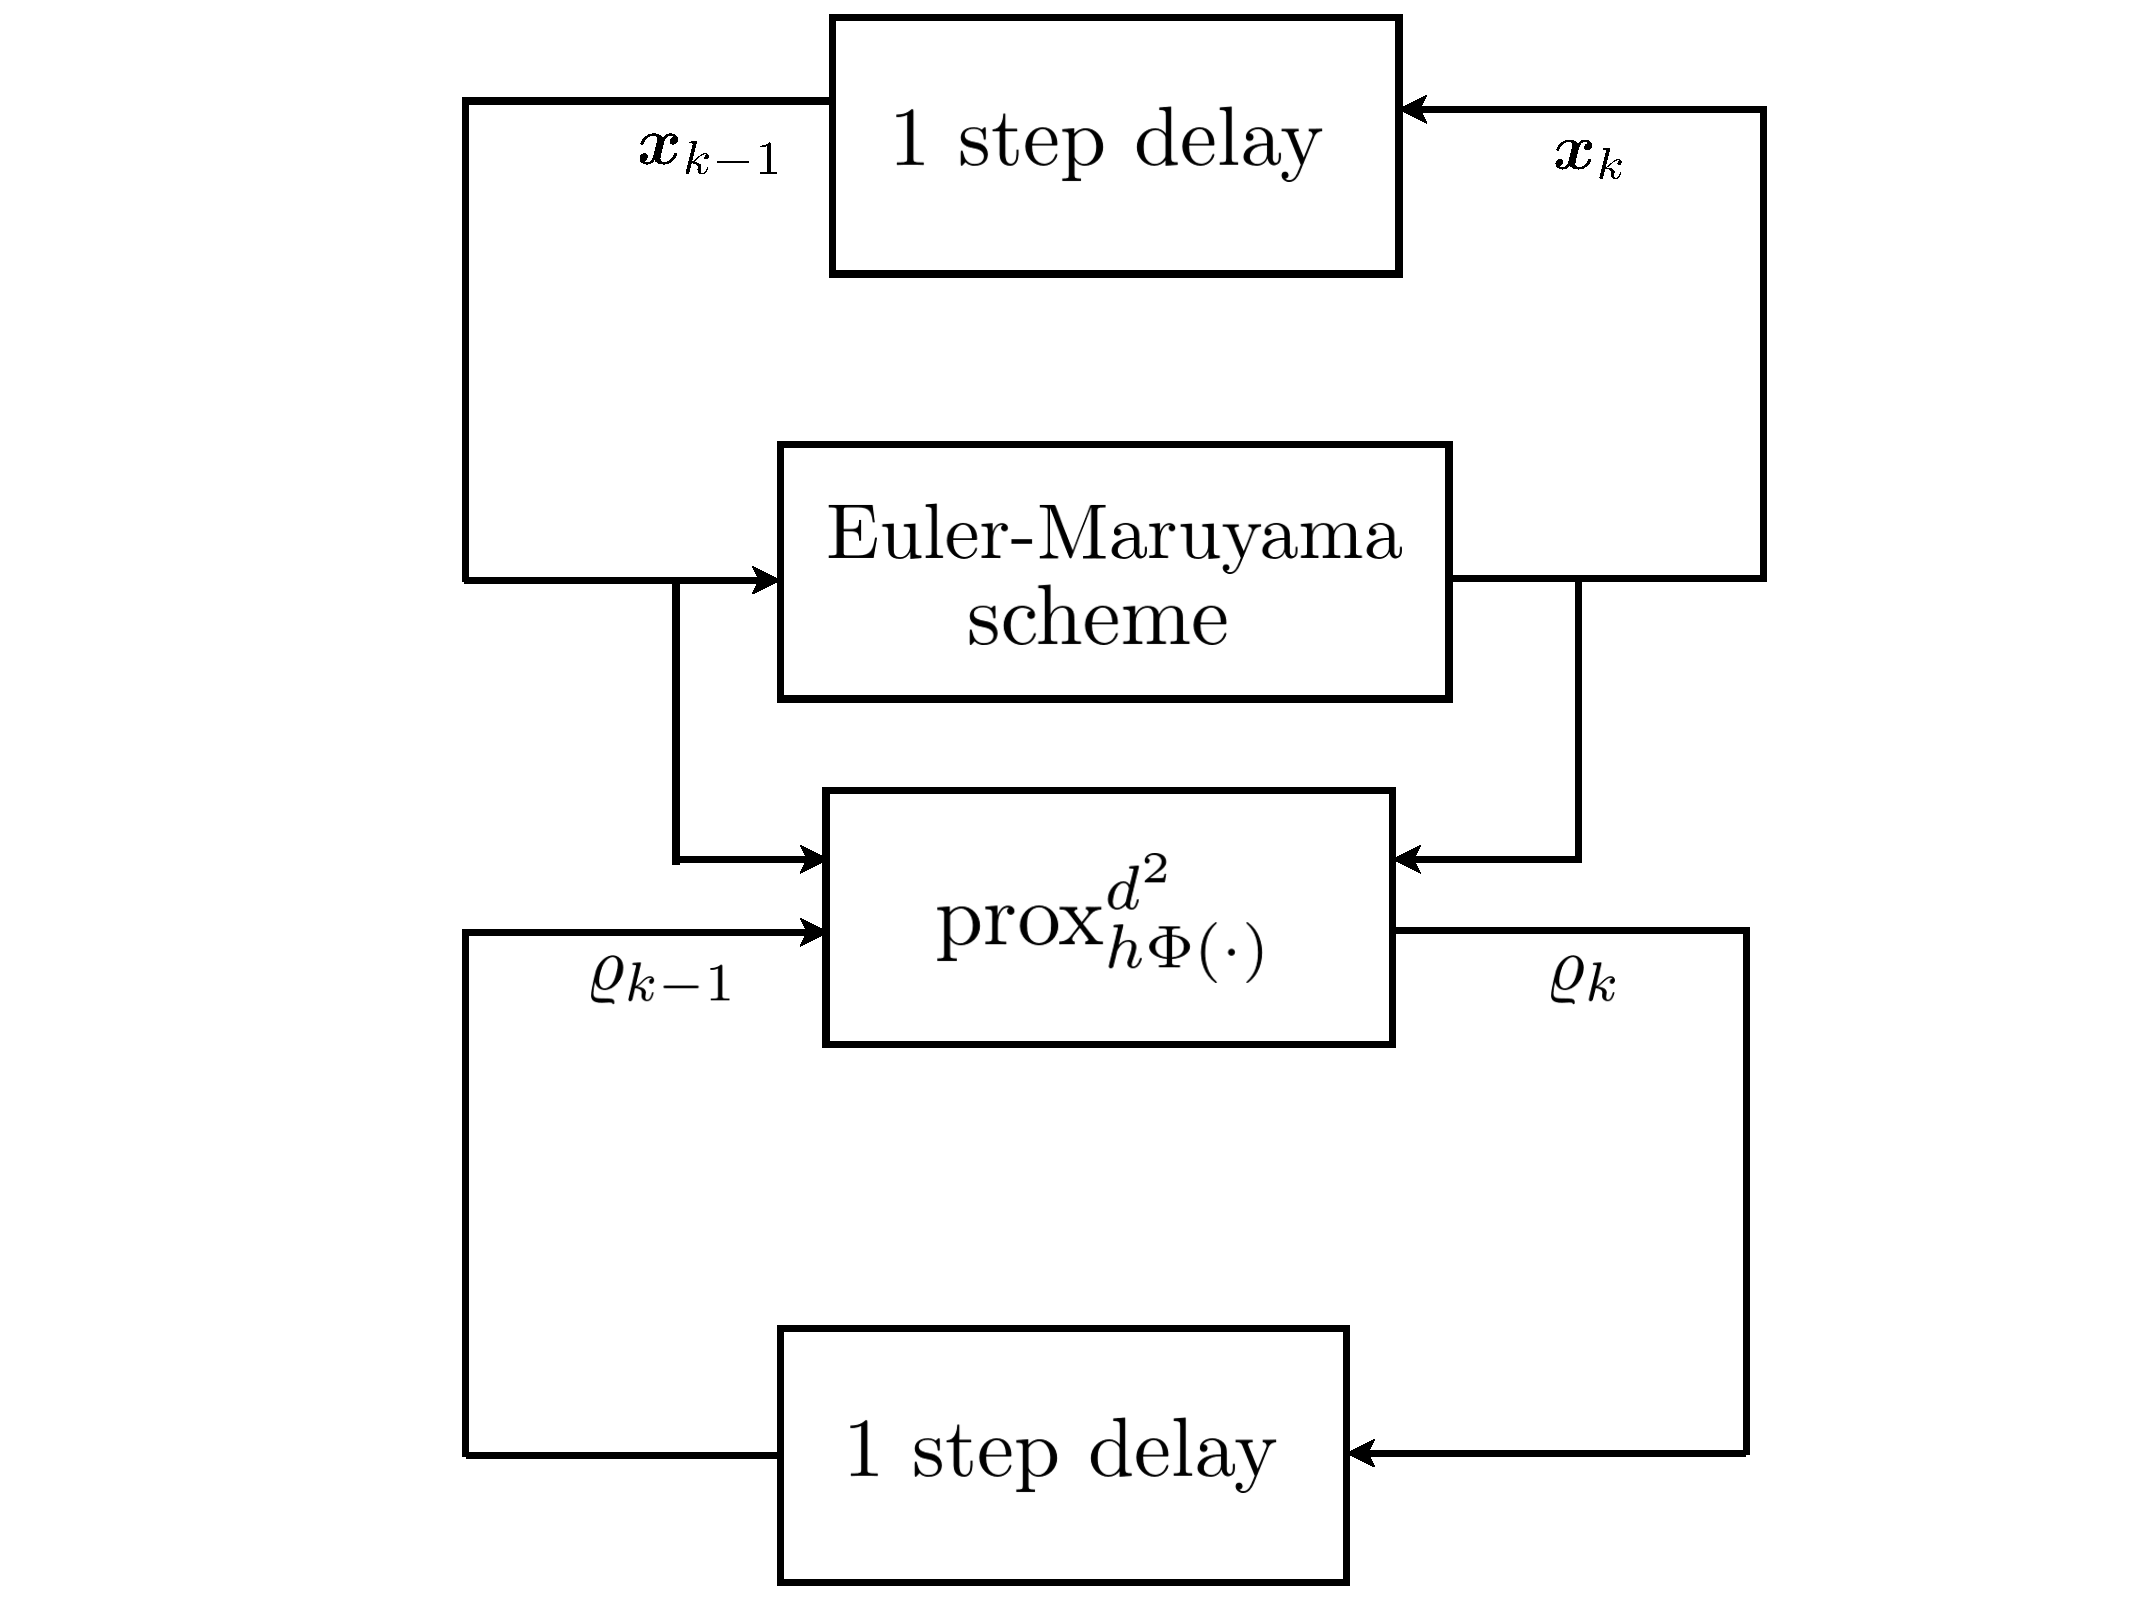
\includegraphics[width=.8\linewidth]{BlockDiagm.pdf}
\caption{\small{Schematic of the proposed algorithmic setup for propagating the joint state PDF as probability weighted scattered point cloud $\{\bm{x}_{k}^{i},\varrho_{k}^{i}\}_{i=1}^{N}$. The location of the points $\{\bm{x}_{k}^{i}\}_{i=1}^{N}$ can be updated by Euler-Maruyama scheme applied to (\ref{ItoSDEvectorlevel}); the corresponding probability weights $\{\varrho_{k}^{i}\}_{i=1}^{N}$ can be updated via discrete version of the proximal recursion (\ref{ProxRecursionInfiniteDim}).}}
\label{fig:BlockDiagm}
\end{figure}


\begin{thebibliography}{99}

\bibitem{villani2003topics}
C. Villani, \emph{Topics in optimal transportation}, No. 58, American Mathematical Society, 2003.
	
\end{thebibliography}


\begin{IEEEbiography}{Michael Shell}
Biography text here.
\end{IEEEbiography}


% insert where needed to balance the two columns on the last page with
% biographies
%\newpage

\begin{IEEEbiography}[{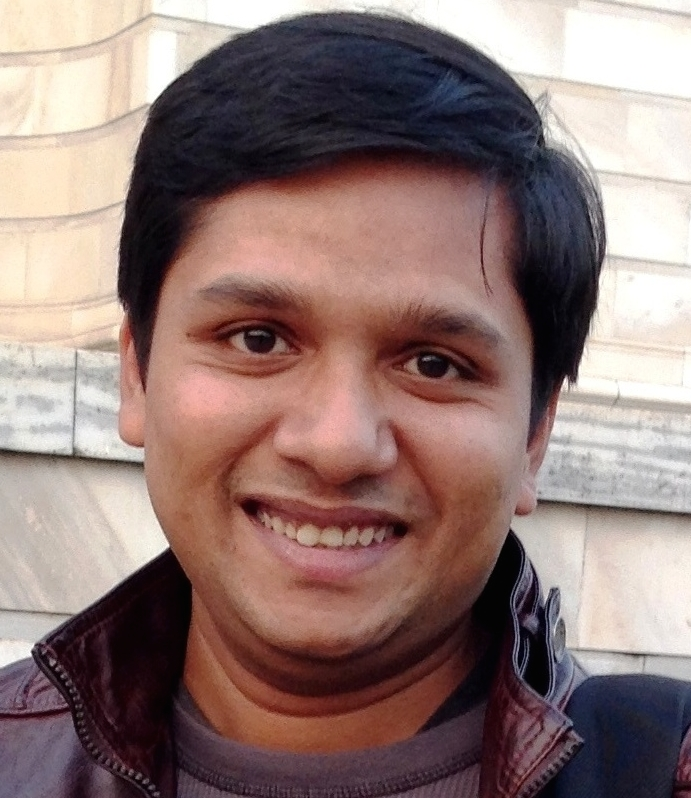
\includegraphics[height=1.25in]{Abhishek-Halder.jpg}}]{Abhishek
Halder}
(S'10-M'14) is an Assistant Professor in the Department of Applied Mathematics,
and is an affiliated faculty in the Department of Electrical and Computer Engineering at
University of California, Santa Cruz. Before that he held postdoctoral
positions in the Department of Mechanical and Aerospace Engineering at
University of California, Irvine, and in the Department of Electrical
and Computer Engineering at Texas A\&M University. He obtained his
Bachelors and Masters from Indian Institute of Technology Kharagpur in
2008, and Ph.D. from Texas A\&M University in 2014, all in Aerospace
Engineering. His research interests are in stochastic systems, control
and optimization with application focus on large scale cyber-physical
systems.
\end{IEEEbiography}

% You can push biographies down or up by placing
% a \vfill before or after them. The appropriate
% use of \vfill depends on what kind of text is
% on the last page and whether or not the columns
% are being equalized.

%\vfill

% Can be used to pull up biographies so that the bottom of the last one
% is flush with the other column.
%\enlargethispage{-5in}



% that's all folks
\end{document}


